%%%%%%%%%%%%%%%%%%%%%%%%%%%%%%%%%%%%%%%%%
% Structured General Purpose Assignment
% LaTeX Template
%
% This template has been downloaded from:
% http://www.latextemplates.com
%
% Original author:
% Ted Pavlic (http://www.tedpavlic.com)
%
% Note:
% The \lipsum[#] commands throughout this template generate dummy text
% to fill the template out. These commands should all be removed when
% writing assignment content.
%
%%%%%%%%%%%%%%%%%%%%%%%%%%%%%%%%%%%%%%%%%

%----------------------------------------------------------------------------------------
%	PACKAGES AND OTHER DOCUMENT CONFIGURATIONS
%----------------------------------------------------------------------------------------

\documentclass{article}

\usepackage{multirow}
\usepackage{amssymb}
\usepackage[fleqn]{amsmath}
\usepackage{url}

\usepackage{fancyhdr} % Required for custom headers
\usepackage{lastpage} % Required to determine the last page for the footer
\usepackage{extramarks} % Required for headers and footers
\usepackage{graphicx} % Required to insert images
\usepackage{lipsum} % Used for inserting dummy 'Lorem ipsum' text into the template

% Margins
\topmargin=-0.45in
\evensidemargin=0in
\oddsidemargin=0in
\textwidth=6.5in
\textheight=9.0in
\headsep=0.25in

\linespread{1.1} % Line spacing

% Set up the header and footer
\pagestyle{fancy}
\lhead{\hmwkAuthorName} % Top left header
\chead{\hmwkClass\ : \hmwkTitle} % Top center header
\rhead{\firstxmark} % Top right header
\lfoot{\lastxmark} % Bottom left footer
\cfoot{} % Bottom center footer
\rfoot{Page\ \thepage\ of\ \pageref{LastPage}} % Bottom right footer
\renewcommand\headrulewidth{0.4pt} % Size of the header rule
\renewcommand\footrulewidth{0.4pt} % Size of the footer rule

\setlength\parindent{0pt} % Removes all indentation from paragraphs

%----------------------------------------------------------------------------------------
%	DOCUMENT STRUCTURE COMMANDS
%	Skip this unless you know what you're doing
%----------------------------------------------------------------------------------------

% Header and footer for when a page split occurs within a problem environment
\newcommand{\enterProblemHeader}[1]{
\nobreak\extramarks{#1}{#1 continued on next page\ldots}\nobreak
\nobreak\extramarks{#1 (continued)}{#1 continued on next page\ldots}\nobreak
}

% Header and footer for when a page split occurs between problem environments
\newcommand{\exitProblemHeader}[1]{
\nobreak\extramarks{#1 (continued)}{#1 continued on next page\ldots}\nobreak
\nobreak\extramarks{#1}{}\nobreak
}

\setcounter{secnumdepth}{0} % Removes default section numbers
\newcounter{homeworkProblemCounter} % Creates a counter to keep track of the number of problems

\newcommand{\homeworkProblemName}{}
\newenvironment{homeworkProblem}[1][Problem \arabic{homeworkProblemCounter}]{ % Makes a new environment called homeworkProblem which takes 1 argument (custom name) but the default is "Problem #"
\stepcounter{homeworkProblemCounter} % Increase counter for number of problems
\renewcommand{\homeworkProblemName}{#1} % Assign \homeworkProblemName the name of the problem
\section{\homeworkProblemName} % Make a section in the document with the custom problem count
\enterProblemHeader{\homeworkProblemName} % Header and footer within the environment
}{
\exitProblemHeader{\homeworkProblemName} % Header and footer after the environment
}

\newcommand{\problemAnswer}[1]{ % Defines the problem answer command with the content as the only argument
\noindent\framebox[\columnwidth][c]{\begin{minipage}{0.98\columnwidth}#1\end{minipage}} % Makes the box around the problem answer and puts the content inside
}

\newcommand{\homeworkSectionName}{}
\newenvironment{homeworkSection}[1]{ % New environment for sections within homework problems, takes 1 argument - the name of the section
\renewcommand{\homeworkSectionName}{#1} % Assign \homeworkSectionName to the name of the section from the environment argument
\subsection{\homeworkSectionName} % Make a subsection with the custom name of the subsection
\enterProblemHeader{\homeworkProblemName\ [\homeworkSectionName]} % Header and footer within the environment
}{
\enterProblemHeader{\homeworkProblemName} % Header and footer after the environment
}

%----------------------------------------------------------------------------------------
%	NAME AND CLASS SECTION
%----------------------------------------------------------------------------------------

\newcommand{\hmwkTitle}{Assignment\ \#2} % Assignment title
\newcommand{\hmwkDueDate}{March\ 11,\ 2016} % Due date
\newcommand{\hmwkClass}{Algorithms} % Course/class
\newcommand{\hmwkAuthorName}{Zhaoyang Li (2014013432)} % Your name

%----------------------------------------------------------------------------------------
%	TITLE PAGE
%----------------------------------------------------------------------------------------

\title{
\vspace{2in}
\textmd{\textbf{\hmwkClass:\ \hmwkTitle}}\\
\normalsize\vspace{0.1in}\small{Due\ on\ \hmwkDueDate}\\
\vspace{3in}
}

\author{\textbf{\hmwkAuthorName}}
\date{} % Insert date here if you want it to appear below your name

%----------------------------------------------------------------------------------------

\begin{document}

\maketitle

%----------------------------------------------------------------------------------------
%	TABLE OF CONTENTS
%----------------------------------------------------------------------------------------

%\setcounter{tocdepth}{1} % Uncomment this line if you don't want subsections listed in the ToC

\newpage
\tableofcontents
\newpage

%----------------------------------------------------------------------------------------
%	PROBLEM 1
%----------------------------------------------------------------------------------------

\begin{homeworkProblem}
Solve planer case of the Closest pair of points problem, in $\Theta(n \lg n)$ time.

\begin{homeworkSection}{Implemantetion} % Section within problem
\problemAnswer{
Both an $\Theta(n \lg n)$ divide-and-conquer algorithm and an $\Theta(n^2)$ brute-force algorithm are implemented, in C++.

For code, please refer to \url{/code/Closest-Pair Problem/}.

Correctness is verified by running both of the implemented algorithms against randomly generated sets of points, and checking if their results contradicts. I got 100\% correctness.

Test\footnote{on an Intel Core i5 4120U Processor, 4GB DDR3 Memory, Windows 10 Pro. Hereinafter the same.} suggests that for $n=10^6$, the $\Theta(n \lg n)$ algorithm takes less than 1 seconds, while the $\Theta(n^2)$ algorithm seems to take forever.
}
\end{homeworkSection}

%--------------------------------------------

\begin{homeworkSection}{Interactive GUI} % Section within problem
\problemAnswer{
Written in C\# WPF, calling pre-compiled DLL where the algorithm is implemented in C++. To be built with Visual Studio 2012.

For code generating the DLL, see \url{/code/Library}. For code building GUI, see \url{/code/Gui}.

Please execute \url{/code/Release/Gui.exe} in Windows to bring up the GUI. Click to add a point. To clear the canvas, restart the program.

}
\end{homeworkSection}


%--------------------------------------------
\begin{homeworkSection}{Timing Comparison} % Section within problem


\problemAnswer{ % Answer
\begin{center}

CPU Time Consumed (microseconds)


\begin{tabular}{rrr}
\hline
Size of the set& $\Theta(n \lg n)$& $\Theta(n^2)$\\
\hline
2 & 0.54 & 0.47 \\
4 & 1.53 & 0.76 \\
8 & 2.43 & 1.18 \\
16 & 5 & 2 \\
32 & 11 & 6 \\
64 & 26 & 13 \\
128 & 54 & 35 \\
256 & 111 & 123 \\
512 & 253 & 440 \\
1024 & 500 & 2000 \\
2048 & 1200 & 7200 \\
4096 & 2600 & 30400 \\
8192 & 5900 & 110300 \\
16384 & 11000 & 438000 \\
32768 & 22000 & 1.72e6 \\
65536 & 73000 & 7.41e6 \\
131072 & 96000 & 2.9e7 \\
... & ... & ... \\
1048576 & 919000 & ?\\
\hline
\end{tabular}

\end{center}
Seems that the cross-over point is somewhere between 128 and 256.

A double-logarithmic chart visualizing the data above:
\begin{center}
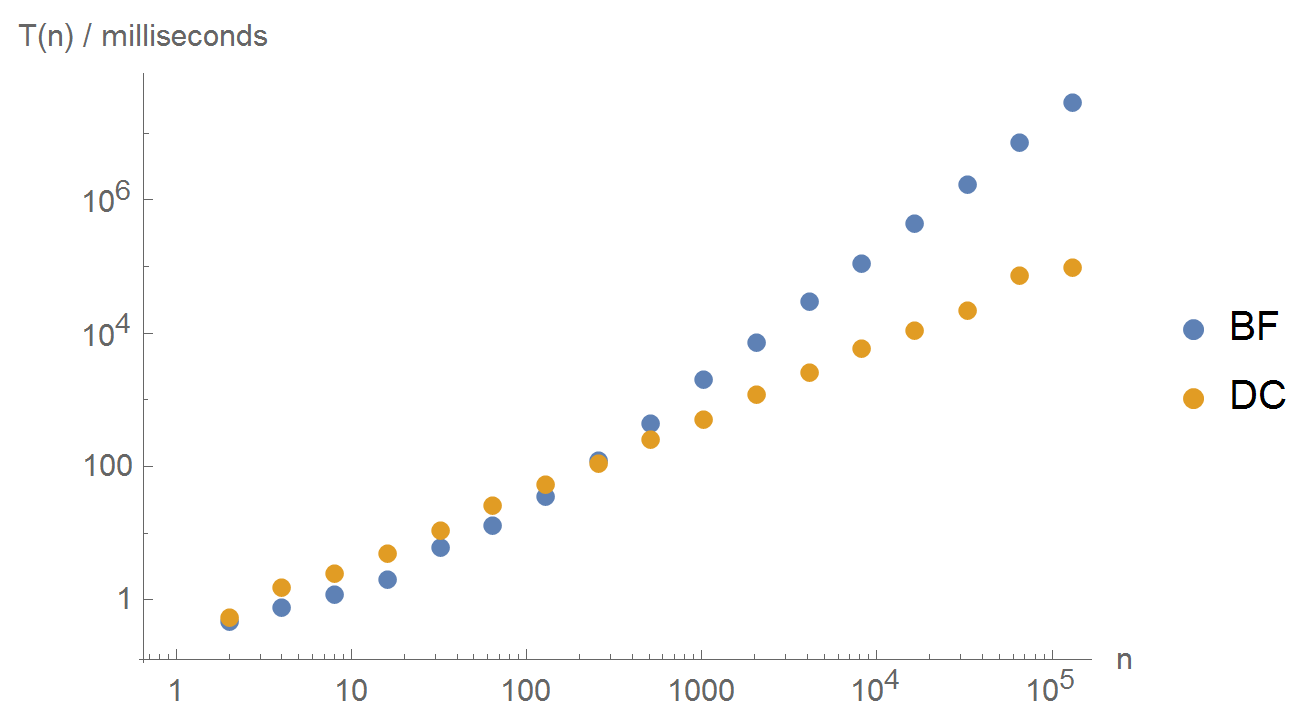
\includegraphics[width=0.75\columnwidth]{chart}
\end{center}



}

\end{homeworkSection}
\end{homeworkProblem}

%----------------------------------------------------------------------------------------
%	PROBLEM 2
%----------------------------------------------------------------------------------------

\begin{homeworkProblem}
CLRS Ex 5.3-5:

Prove that in the array P in procedure PERMUTE-BY-SORTING, the probability that all elements are unique is at least $1-\frac{1}{n}$.

\problemAnswer{
Proof:

Let A = \{all elements are unique\}.

$$n(\Omega) = (n^3)^n$$

$$n(A) = A_{n^3}^n$$

Applying classical probability model, possibility of A

\[
\begin{aligned}
P\left( A\right)  & =\frac{n\left( A\right) }{n\left( \Omega\right) } \\
& = \frac{A_{n^3}^n}{\left( n^3\right) ^n} \\
& = \frac{\left( n^3\right) !}{\left( n^3-n\right) ! n^{3n}}\\
& = \prod_{i=0}^{n-1} \frac{n^3-i}{n^3}\\
& > \prod_{i=0}^{n-1} \frac{n^3-n}{n^3}\\
& = \prod_{i=0}^{n-1} \left( 1-\frac{1}{n^2}\right) \\
& = \left( 1-\frac{1}{n^2}\right) ^n\\
\end{aligned}
\]

Applying binomial theorem where $a=1, b=-\frac{1}{n^2}$,

\[
\begin{aligned}
P\left( A\right)  & > \left( 1-\frac{1}{n^2}\right) ^n\\
& = \sum_{i=0}^{n} C_n^i \left( -\frac{1}{n^2}\right) ^{i}\\
& = 1 - \frac{1}{n} + \sum_{i=2}^{n} C_n^i \left( -\frac{1}{n^2}\right) ^{i}\\
& \ge 1 - \frac{1}{n} + \sum_{j=1}^{\lfloor\frac{n-1}{2}\rfloor} C_n^{2j} \left( \left( -\frac{1}{n^2}\right) ^{2j}+\left( -\frac{1}{n^2}\right) ^{2j+1}\right) \\
& = 1 - \frac{1}{n} + \sum_{j=1}^{\lfloor\frac{n-1}{2}\rfloor} C_n^{2j} \left( \frac{1}{n^{4j}}-\frac{1}{n^{4j+2}}\right) \\
& \ge 1 - \frac{1}{n}
\end{aligned}
\]


QED.


}

%--------------------------------------------


%--------------------------------------------

\end{homeworkProblem}



%----------------------------------------------------------------------------------------

\end{document}
